\chapter{B:分析迭代客户满意度调查数据} % Introduction chapter suppressed from the table of contents

\hypertarget{ux6848ux4f8bux80ccux666f}{%
\subsection{案例背景}\label{ux6848ux4f8bux80ccux666f}}

香港公司在广州的离岸软件开发中心,专门为香港的客户,如政府部门,做软件维护工作。从2019年,项目已经开始采用
SCRUM
敏捷开发方式,每两周一个冲刺,他们每次做完迭代后,客户都会填写满意度调查,然后分析数据。

\hypertarget{ux8fedux4ee3ux6570ux636e}{%
\subsection{迭代数据}\label{ux8fedux4ee3ux6570ux636e}}

每次迭代团队都会收集以下数据:

\begin{itemize}
\tightlist
\item
  客户满意度调查(Cust Sat survey)
\item
  需求变更请求次数(Requirements and Change Requests)
\item
  系统测试缺陷数(Test defects)
\end{itemize}

\hypertarget{ux6570ux636eux5206ux6790}{%
\subsection{数据分析}\label{ux6570ux636eux5206ux6790}}

\begin{itemize}
\tightlist
\item
  Overall满意度(整体指标)与7\textasciitilde{}8个因素相关,而与其中的Deliverable
  Quality相关系数达到0.90,Deliverable Time
  0.688左右,其他的相关性都较低。
\end{itemize}

%\href{文件:微信截图_20230625135709.png}{600px\textbar{}无}

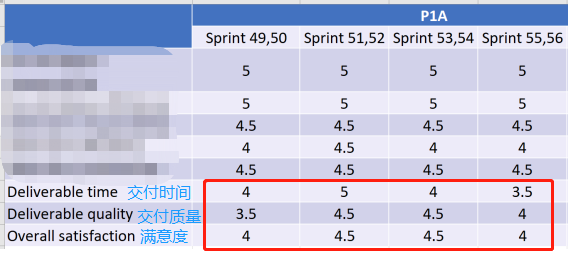
\includegraphics[width=6cm]{微信截图_20230625135709.png}

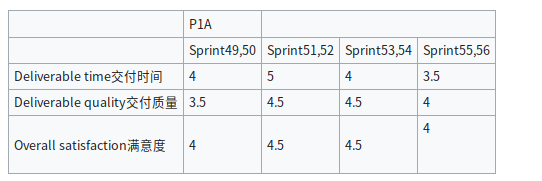
\includegraphics[width=6cm]{Screenshotfrom2023-10-1223-17-39.png}
%Screenshotfrom2023-10-1223-17-39.png

\begin{itemize}
\tightlist
\item
  测试缺陷数和以下客户行为相关性如下:插入任务 0.51,需求模糊
  0.66,初期没有需求问题 -0.45,需求不稳定引起返工 0.82。(详见下图)
\end{itemize}

(为什么初期需求模糊反而是-0.45:等需求明确,写成文档,导致后期才能给明确需求,反而比早期给个模糊需求好,因更可能引起返工。)

%\href{文件:微信截图_20230625135338.png}{600px\textbar{}无}

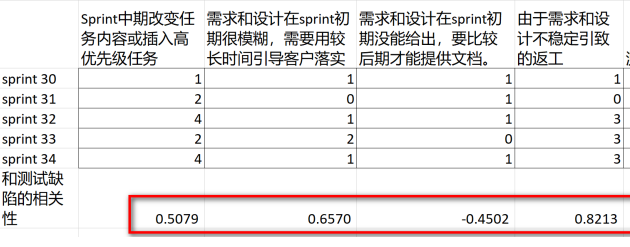
\includegraphics[width=6cm]{微信截图_20230625135338.png}

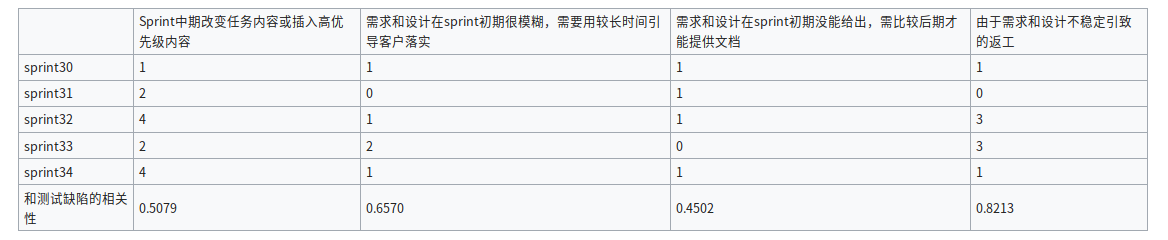
\includegraphics[width=6cm]{Screenshotfrom2023-10-1223-18-56.png}

若能写好需求,减少插入任务和变更,可以提升质量(降低测试缺陷数)。

\hypertarget{ux6539ux8fdbux63aaux65bd}{%
\subsection{改进措施}\label{ux6539ux8fdbux63aaux65bd}}

\begin{itemize}
\tightlist
\item
  固化Clarification流程。当前是较为随机,由开发人员发起(统计数据中每个迭代0\textasciitilde{}2次),后面优化Clarification
  过程,要求每次迭代都必须做需求Clarification,形式也更正式,明确甲乙双方哪些岗位、什么角色必须参与,在确认新过程有效后,就把过程固化下来。
\item
  把需求 Clarification 要具备的重点写成检查单,增加检查项,如:

  \begin{itemize}
  \tightlist
  \item
    需求是否完整明确
  \item
    是否按简化功能点方法写清行为、实体
  \item
    场景是否明确
  \item
    能否有对应明确测试用例(是否可测试)
  \end{itemize}
\item
  请甲方尽量减少插入任务和变更。
\end{itemize}

\hypertarget{ux6539ux8fdbux6548ux679c}{%
\subsection{改进效果}\label{ux6539ux8fdbux6548ux679c}}

除了客户满意度得到提升外,冲刺生产率也提升,例如:\\
生产率之前四分位数是 (1.07, 1.13, 1.16)
,采取控制插入任务,减少变更,做好Clarification等措施后,有明显改善,变为
(1.04, 1.05 , 1.08) 。\\
(注: 它们生产率 = 人天/功能点数 , 所以生产率系数是越低越好)

